\documentclass{article}

\usepackage{graphicx}
\usepackage{blindtext}

\title{LATEX EJEMPLOS CON FIGURAS}

\begin{document}
    \maketitle
   \blindtext[2]\\


 %%%%%%%%%%%%%%%%%%%%%%%%%%%%%%%%%%%%%%%%%%%%%%%%%
    \begin{figure}[ht]
    %\hspace{0mm}
        \begin{flushright}
            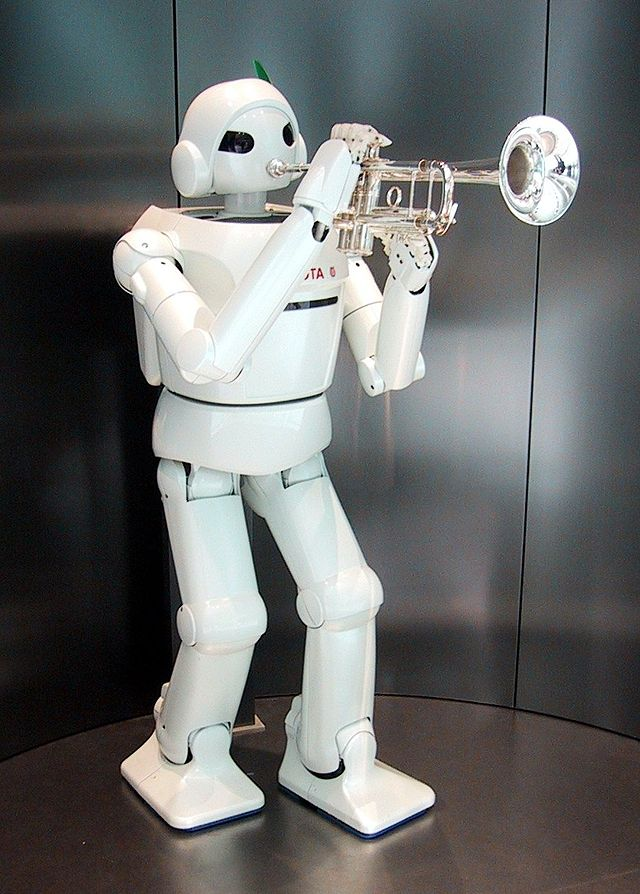
\includegraphics[scale=0.3]{robot1.jpg}
            \caption{Un robot musical}
            \label{robot1}
        \end{flushright}
    \end{figure}


    \blindtext[10]
%%%%%%%%%%%%%%%%%%%%%%%%%%%%%%%%%%%%%%%%%%%%%%%
    \begin{figure}[t]
        \centering
        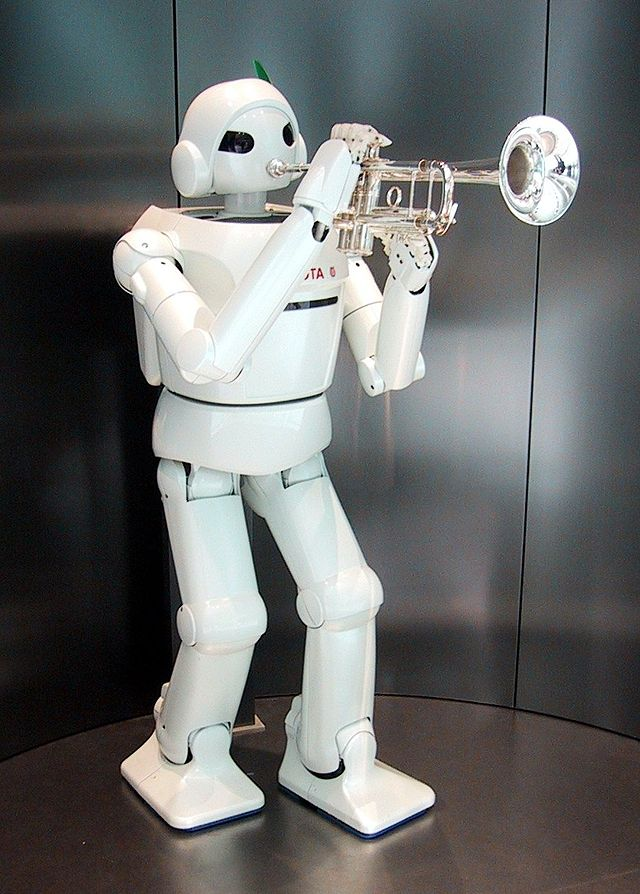
\includegraphics[width=6.0cm]{robot1.jpg}
        
\includegraphics[width=6.0cm]{robot2.jpeg}
        \caption{A robot1 y robot 2.}
        \label{robots pegados}
    \end{figure}

\blindtext[10]
%%%%%%%%%%%%%%%%%%%%%%%%%%%%%%%%%%%%%%%%%%%%%%%%%%%
    \begin{figure}[b]
        \begin{minipage}[c]{.6\linewidth}
            \centering
            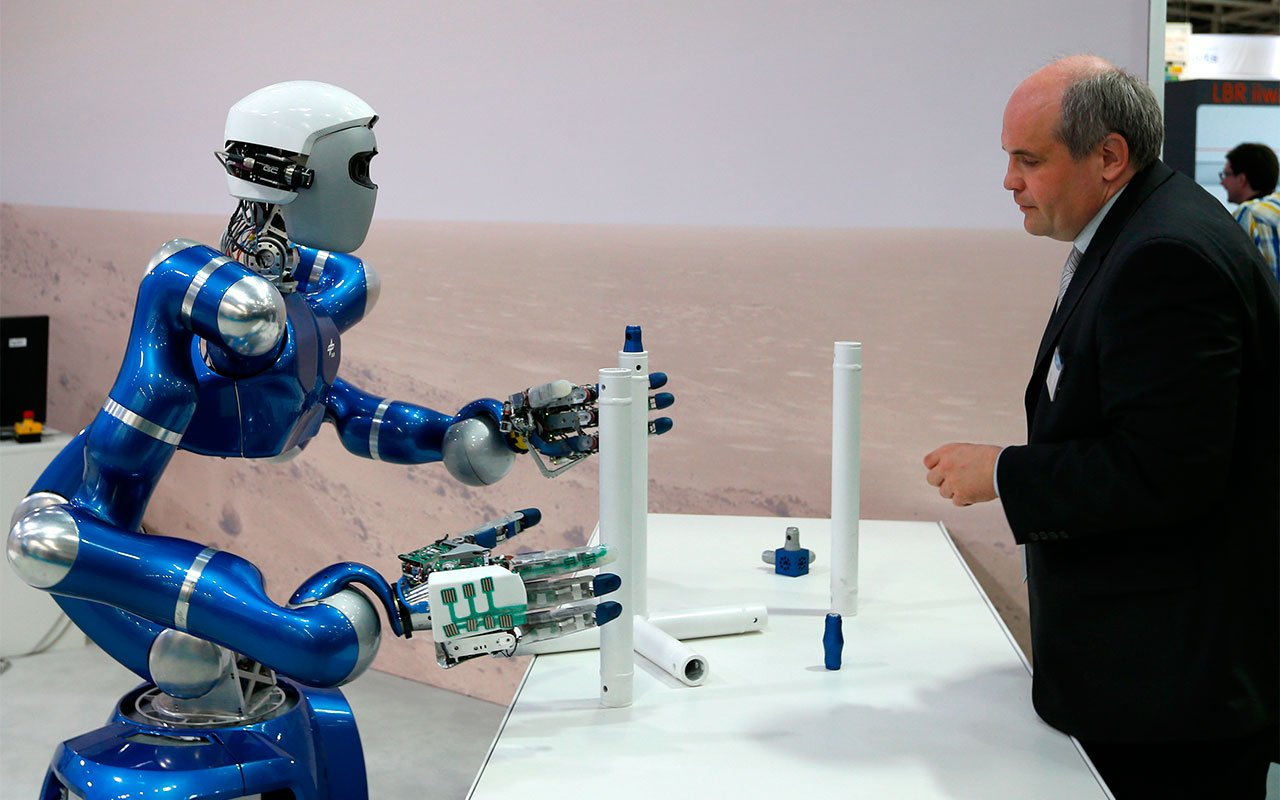
\includegraphics[width=6.0cm]{robot4.jpg}
            \caption{A girl.}
            \label{girl}
        \end{minipage}\hfill
%
        \begin{minipage}[c]{.6\linewidth}
            \centering
            
\includegraphics[width=6cm]{robot2.jpeg}
            \caption{A flower.}
            \label{flower}
        \end{minipage}
       
    \end{figure}
%%%%%%%%%%%%%%%%%%%%%%%%%%%%%%%%%%%%%%%%%%%%%%%%%%%
\blindtext[10]
\end{document}